



\chapter{Conclusions and Future Work} \label{chap:concl}

\section*{}


\section{Data exploration and analysis}

Upon close examination of the data summary, we can surmise that the classification for the two states is unbalanced. \ref{tab:2StatesClassification} .

And it turns out that there are fields with null values, 111 in total. This happens when the patient is blind or the gustatory sensory system is not possible to assess. It happens in the situations like patients are fed through a gastric tube or other alternative feeding mechanisms such as transcheostemia, etc.
All 'NA' are changed and assigned a non-significant value: -1. 
The reason for doing so is that data is precious and scarce, and removing records would further shorten our dataset. If we do not have sufficient. 
Without data, you cannot make the algorithm make a perfect model.
The ID and order insignificant columns are removed.
And the column of the diagnosis made by human evaluators, our label, is separated from X for an isolated panda's series y.

\section{Machine Learning}

X and y are split into training and testing subsets.
Taking care to stratify the data in relation to the label (stratify=y).
This is to ensure that all classes are proportional in relation to the training side to the testing side, avoiding the risk of poorly trained classes.
\clearpage

\section{Results}

The project repository is available at: https://github.com/ManJ-PC/ML-DoC

\espaco
\begin{figure}[ht] \centering 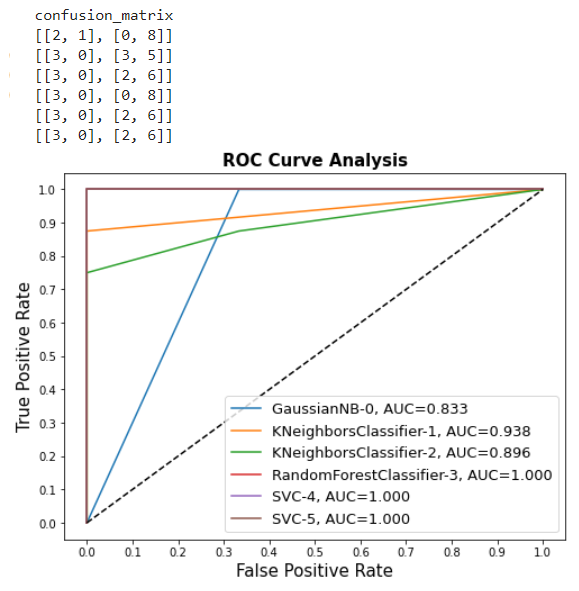
\includegraphics[scale=0.5]{figures/Results.png} 
\caption{Confusion Matrix and ROC curve of a Bunch of Algorithms} \label{fig:results}
 \end{figure}
 

\begin{figure}[ht] \centering 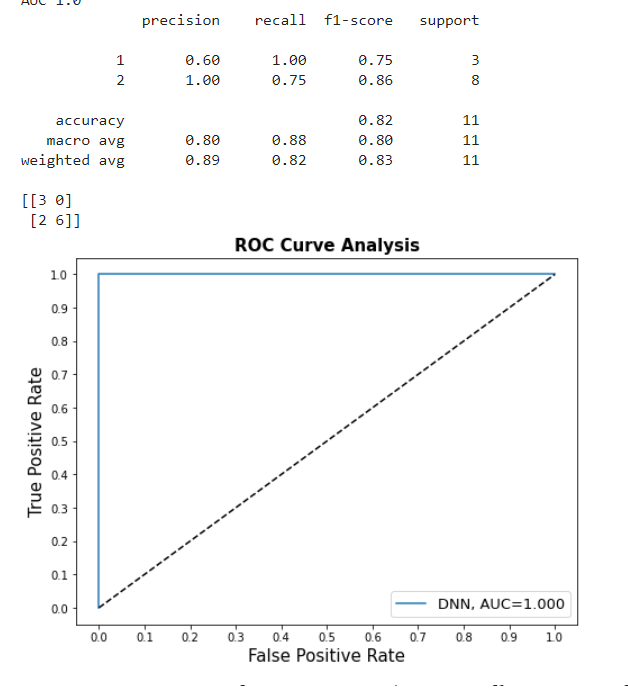
\includegraphics[scale=0.5]{figures/ResultsNN.png} 
\caption{Neural Network, Confusion Matrix and ROC curve resulting from the iterative method with 100 epochs, 25 neurons and ADAM optimizer} \label{fig:resultsNN}
 \end{figure}
 

\section{Further Work}



The project can be futher developed to find correlation of features in algorithms. Divide in two subgroups based on etiology. We can also see if it is possible to do less sessions to minimize resources of this tecnique(human resources, time spend). Since it may no longer be adding added value to the data.
\begin{itemize}
\item A broader view of classification in 3 possible stages (vegetative state, minimal state of consciousness minus and plus)
\item Iterate over the various machine learning algorithms
\item Unification of similar features \cite{9202409}
\item Predict the correlation of selected features and limit the number of sessions needed
\item Use of diagnostic tools to sensory data acquisition
\item Test the model with new and real data where it does not contain as rather sessions
\item Automate the entire process, acquire technological tools that allow you to track patients regularly
\end{itemize}


\vspace*{12mm}


